% Options for packages loaded elsewhere
\PassOptionsToPackage{unicode}{hyperref}
\PassOptionsToPackage{hyphens}{url}
%
\documentclass[
]{article}
\usepackage{amsmath,amssymb}
\usepackage{lmodern}
\usepackage{ifxetex,ifluatex}
\ifnum 0\ifxetex 1\fi\ifluatex 1\fi=0 % if pdftex
  \usepackage[T1]{fontenc}
  \usepackage[utf8]{inputenc}
  \usepackage{textcomp} % provide euro and other symbols
\else % if luatex or xetex
  \usepackage{unicode-math}
  \defaultfontfeatures{Scale=MatchLowercase}
  \defaultfontfeatures[\rmfamily]{Ligatures=TeX,Scale=1}
\fi
% Use upquote if available, for straight quotes in verbatim environments
\IfFileExists{upquote.sty}{\usepackage{upquote}}{}
\IfFileExists{microtype.sty}{% use microtype if available
  \usepackage[]{microtype}
  \UseMicrotypeSet[protrusion]{basicmath} % disable protrusion for tt fonts
}{}
\makeatletter
\@ifundefined{KOMAClassName}{% if non-KOMA class
  \IfFileExists{parskip.sty}{%
    \usepackage{parskip}
  }{% else
    \setlength{\parindent}{0pt}
    \setlength{\parskip}{6pt plus 2pt minus 1pt}}
}{% if KOMA class
  \KOMAoptions{parskip=half}}
\makeatother
\usepackage{xcolor}
\IfFileExists{xurl.sty}{\usepackage{xurl}}{} % add URL line breaks if available
\IfFileExists{bookmark.sty}{\usepackage{bookmark}}{\usepackage{hyperref}}
\hypersetup{
  pdftitle={Final Project},
  pdfauthor={Zhengtao Xu, Jennings Cheng and Collin Carmichael},
  hidelinks,
  pdfcreator={LaTeX via pandoc}}
\urlstyle{same} % disable monospaced font for URLs
\usepackage[margin=1in]{geometry}
\usepackage{graphicx}
\makeatletter
\def\maxwidth{\ifdim\Gin@nat@width>\linewidth\linewidth\else\Gin@nat@width\fi}
\def\maxheight{\ifdim\Gin@nat@height>\textheight\textheight\else\Gin@nat@height\fi}
\makeatother
% Scale images if necessary, so that they will not overflow the page
% margins by default, and it is still possible to overwrite the defaults
% using explicit options in \includegraphics[width, height, ...]{}
\setkeys{Gin}{width=\maxwidth,height=\maxheight,keepaspectratio}
% Set default figure placement to htbp
\makeatletter
\def\fps@figure{htbp}
\makeatother
\setlength{\emergencystretch}{3em} % prevent overfull lines
\providecommand{\tightlist}{%
  \setlength{\itemsep}{0pt}\setlength{\parskip}{0pt}}
\setcounter{secnumdepth}{-\maxdimen} % remove section numbering
\ifluatex
  \usepackage{selnolig}  % disable illegal ligatures
\fi

\title{Final Project}
\author{Zhengtao Xu, Jennings Cheng and Collin Carmichael}
\date{7/22/2021}

\begin{document}
\maketitle

\textbf{Introduction}

\textbf{Exploratory Data Analysis}

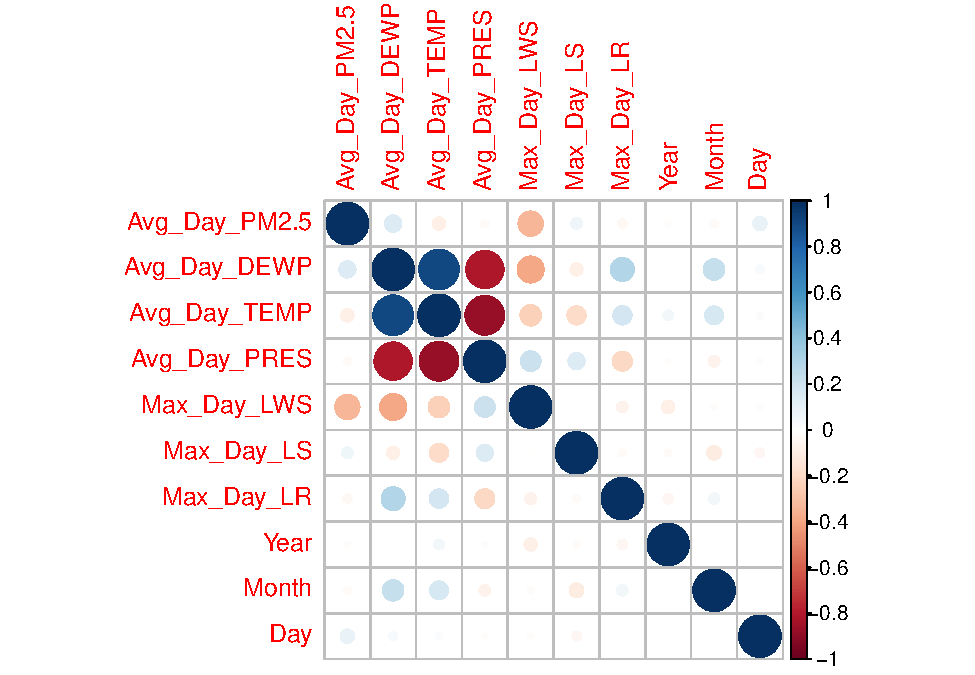
\includegraphics{Final_Project_1_files/figure-latex/unnamed-chunk-3-1.pdf}
Looking at a correlation heatmap we see aside from dewpoint
precipitation and temperature there are no significant correlation in
other variable

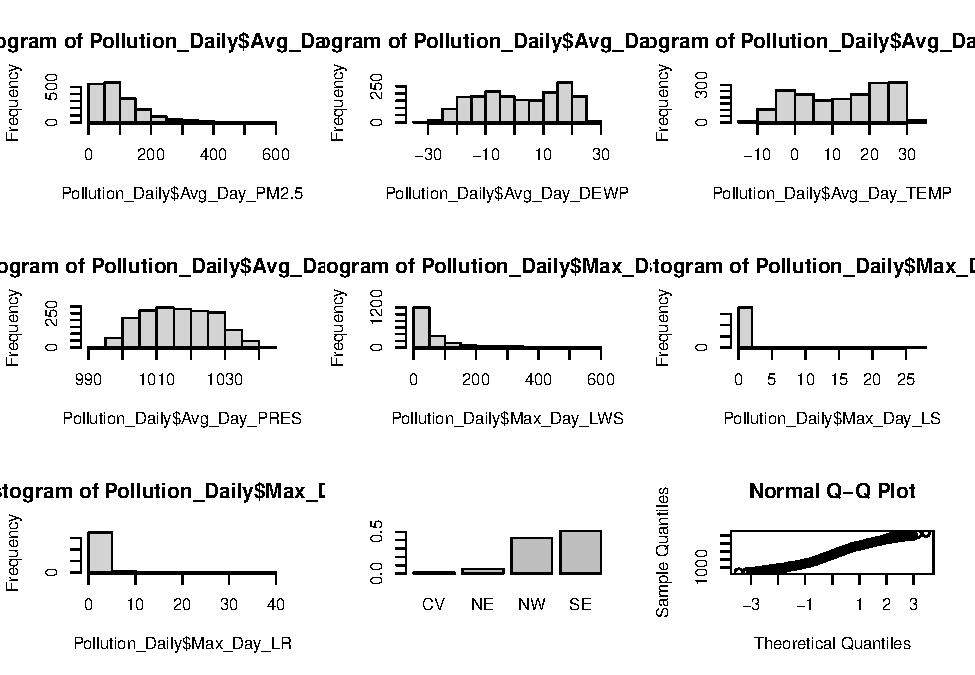
\includegraphics{Final_Project_1_files/figure-latex/unnamed-chunk-4-1.pdf}
We can see that PM2.5 has an inverse distribution with values skewed
towards low PM2.5 but many high values that go beyond the median

Temp and Dew point are highly related and so may not need to be included
in the same model

Precipitation looks like a bell curve but not normal as seen in the plot
in 3,3

Wind speed is similar but not identical to PM2.5 in that it has an
inverse distribution so it may be highly important in prediction

There is almost always not any snow in Beijing and the max is 27 for a
day

Rain is also infrequent but there are times when there is a lot of rain

The most common direction is SE and NW while sometimes NE or CV

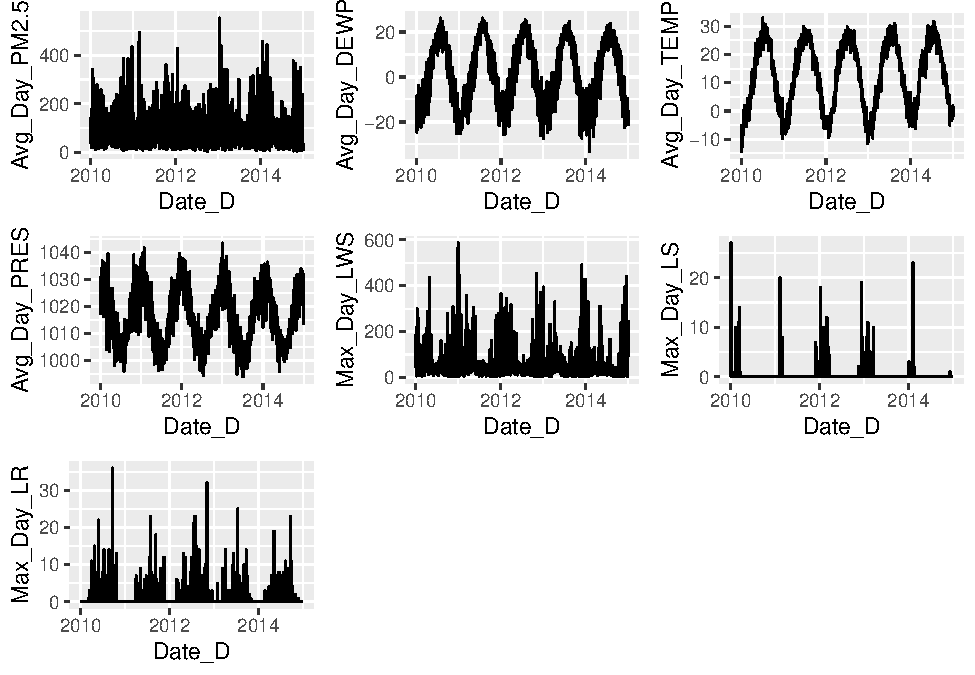
\includegraphics{Final_Project_1_files/figure-latex/unnamed-chunk-5-1.pdf}
We see that pm2.5 varies in a slightly seasonal way in that peaks are
near the start of year while dew point and temperature all peak in
middle and precipitation peak during beginning with snow - wind speed
also are near the time period

One thing that we can do also is based on common sense, we can predict
that PM2.5 will not vary greatly with the day, month or year as we see
that the pm2.5 time series is mostly random spikes with a mean of 200
about so let us see the day month and year

\begin{verbatim}
## 
## Call:
## lm(formula = Avg_Day_PM2.5 ~ ., data = Pollution_Daily.train)
## 
## Residuals:
##     Min      1Q  Median      3Q     Max 
## -159.14  -40.87  -10.04   29.32  321.50 
## 
## Coefficients:
##                  Estimate Std. Error t value Pr(>|t|)    
## (Intercept)    -4.615e+06  2.113e+06  -2.184 0.029089 *  
## Date_D         -6.411e+00  2.935e+00  -2.184 0.029129 *  
## Avg_Day_DEWP    7.189e+00  3.627e-01  19.821  < 2e-16 ***
## Avg_Day_TEMP   -1.081e+01  4.737e-01 -22.824  < 2e-16 ***
## Avg_Day_PRES   -2.504e+00  3.322e-01  -7.539 8.43e-14 ***
## Max_Day_LWS    -1.646e-01  2.730e-02  -6.030 2.08e-09 ***
## Max_Day_LS     -4.196e+00  1.016e+00  -4.132 3.81e-05 ***
## Max_Day_LR     -5.354e+00  6.344e-01  -8.440  < 2e-16 ***
## Max_Day_CBWDNE -7.925e+01  1.803e+01  -4.395 1.19e-05 ***
## Max_Day_CBWDNW -5.632e+01  1.677e+01  -3.359 0.000803 ***
## Max_Day_CBWDSE -5.075e+01  1.670e+01  -3.038 0.002424 ** 
## Year            2.344e+03  1.072e+03   2.186 0.028992 *  
## Month           1.933e+02  8.935e+01   2.163 0.030699 *  
## Day             7.128e+00  2.934e+00   2.430 0.015231 *  
## ---
## Signif. codes:  0 '***' 0.001 '**' 0.01 '*' 0.05 '.' 0.1 ' ' 1
## 
## Residual standard error: 61.18 on 1420 degrees of freedom
##   (因为不存在,26个观察量被删除了)
## Multiple R-squared:  0.4062, Adjusted R-squared:  0.4007 
## F-statistic: 74.71 on 13 and 1420 DF,  p-value: < 2.2e-16
\end{verbatim}

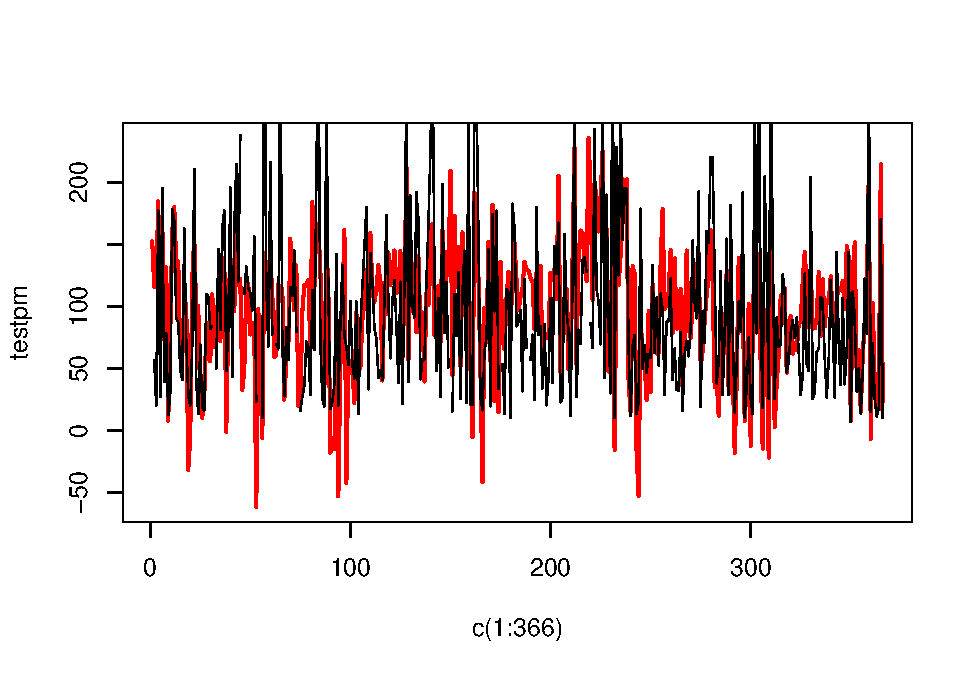
\includegraphics{Final_Project_1_files/figure-latex/unnamed-chunk-7-1.pdf}

\begin{verbatim}
## Warning in axis(side, at = z, labels = labels, ...):
## 'mbcsToSbcs'Àïת»»'周三'³ö´í£º<e5>´úÌæÁËdot
\end{verbatim}

\begin{verbatim}
## Warning in axis(side, at = z, labels = labels, ...):
## 'mbcsToSbcs'Àïת»»'周三'³ö´í£º<91>´úÌæÁËdot
\end{verbatim}

\begin{verbatim}
## Warning in axis(side, at = z, labels = labels, ...):
## 'mbcsToSbcs'Àïת»»'周三'³ö´í£º<a8>´úÌæÁËdot
\end{verbatim}

\begin{verbatim}
## Warning in axis(side, at = z, labels = labels, ...):
## 'mbcsToSbcs'Àïת»»'周三'³ö´í£º<e4>´úÌæÁËdot
\end{verbatim}

\begin{verbatim}
## Warning in axis(side, at = z, labels = labels, ...):
## 'mbcsToSbcs'Àïת»»'周三'³ö´í£º<b8>´úÌæÁËdot
\end{verbatim}

\begin{verbatim}
## Warning in axis(side, at = z, labels = labels, ...):
## 'mbcsToSbcs'Àïת»»'周三'³ö´í£º<89>´úÌæÁËdot
\end{verbatim}

\begin{verbatim}
## Warning in axis(side, at = z, labels = labels, ...):
## 'mbcsToSbcs'Àïת»»'周三'³ö´í£º<e5>´úÌæÁËdot
\end{verbatim}

\begin{verbatim}
## Warning in axis(side, at = z, labels = labels, ...):
## 'mbcsToSbcs'Àïת»»'周三'³ö´í£º<91>´úÌæÁËdot
\end{verbatim}

\begin{verbatim}
## Warning in axis(side, at = z, labels = labels, ...):
## 'mbcsToSbcs'Àïת»»'周三'³ö´í£º<a8>´úÌæÁËdot
\end{verbatim}

\begin{verbatim}
## Warning in axis(side, at = z, labels = labels, ...):
## 'mbcsToSbcs'Àïת»»'周三'³ö´í£º<e4>´úÌæÁËdot
\end{verbatim}

\begin{verbatim}
## Warning in axis(side, at = z, labels = labels, ...):
## 'mbcsToSbcs'Àïת»»'周三'³ö´í£º<b8>´úÌæÁËdot
\end{verbatim}

\begin{verbatim}
## Warning in axis(side, at = z, labels = labels, ...):
## 'mbcsToSbcs'Àïת»»'周三'³ö´í£º<89>´úÌæÁËdot
\end{verbatim}

\begin{verbatim}
## Warning in axis(side, at = z, labels = labels, ...):
## 'mbcsToSbcs'Àïת»»'周四'³ö´í£º<e5>´úÌæÁËdot
\end{verbatim}

\begin{verbatim}
## Warning in axis(side, at = z, labels = labels, ...):
## 'mbcsToSbcs'Àïת»»'周四'³ö´í£º<91>´úÌæÁËdot
\end{verbatim}

\begin{verbatim}
## Warning in axis(side, at = z, labels = labels, ...):
## 'mbcsToSbcs'Àïת»»'周四'³ö´í£º<a8>´úÌæÁËdot
\end{verbatim}

\begin{verbatim}
## Warning in axis(side, at = z, labels = labels, ...):
## 'mbcsToSbcs'Àïת»»'周四'³ö´í£º<e5>´úÌæÁËdot
\end{verbatim}

\begin{verbatim}
## Warning in axis(side, at = z, labels = labels, ...):
## 'mbcsToSbcs'Àïת»»'周四'³ö´í£º<9b>´úÌæÁËdot

## Warning in axis(side, at = z, labels = labels, ...):
## 'mbcsToSbcs'Àïת»»'周四'³ö´í£º<9b>´úÌæÁËdot
\end{verbatim}

\begin{verbatim}
## Warning in axis(side, at = z, labels = labels, ...):
## 'mbcsToSbcs'Àïת»»'周五'³ö´í£º<e5>´úÌæÁËdot
\end{verbatim}

\begin{verbatim}
## Warning in axis(side, at = z, labels = labels, ...):
## 'mbcsToSbcs'Àïת»»'周五'³ö´í£º<91>´úÌæÁËdot
\end{verbatim}

\begin{verbatim}
## Warning in axis(side, at = z, labels = labels, ...):
## 'mbcsToSbcs'Àïת»»'周五'³ö´í£º<a8>´úÌæÁËdot
\end{verbatim}

\begin{verbatim}
## Warning in axis(side, at = z, labels = labels, ...):
## 'mbcsToSbcs'Àïת»»'周五'³ö´í£º<e4>´úÌæÁËdot
\end{verbatim}

\begin{verbatim}
## Warning in axis(side, at = z, labels = labels, ...):
## 'mbcsToSbcs'Àïת»»'周五'³ö´í£º<ba>´úÌæÁËdot
\end{verbatim}

\begin{verbatim}
## Warning in axis(side, at = z, labels = labels, ...):
## 'mbcsToSbcs'Àïת»»'周五'³ö´í£º<94>´úÌæÁËdot
\end{verbatim}

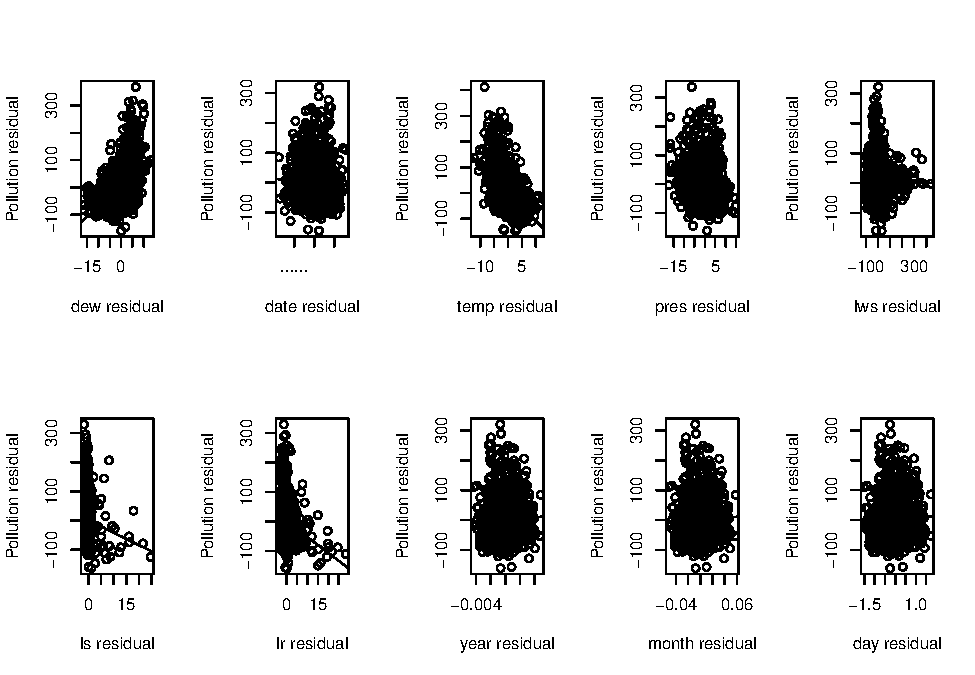
\includegraphics{Final_Project_1_files/figure-latex/unnamed-chunk-7-2.pdf}
After fitting a full model we see every single predictor is significant
however R square is only 0.4 which suggests even though each coefficient
is directionally correct the variation of response is not accurate

Doing a diagnostic of partial regression, There are no normally
distributed partial regression and therefore the model is not linear

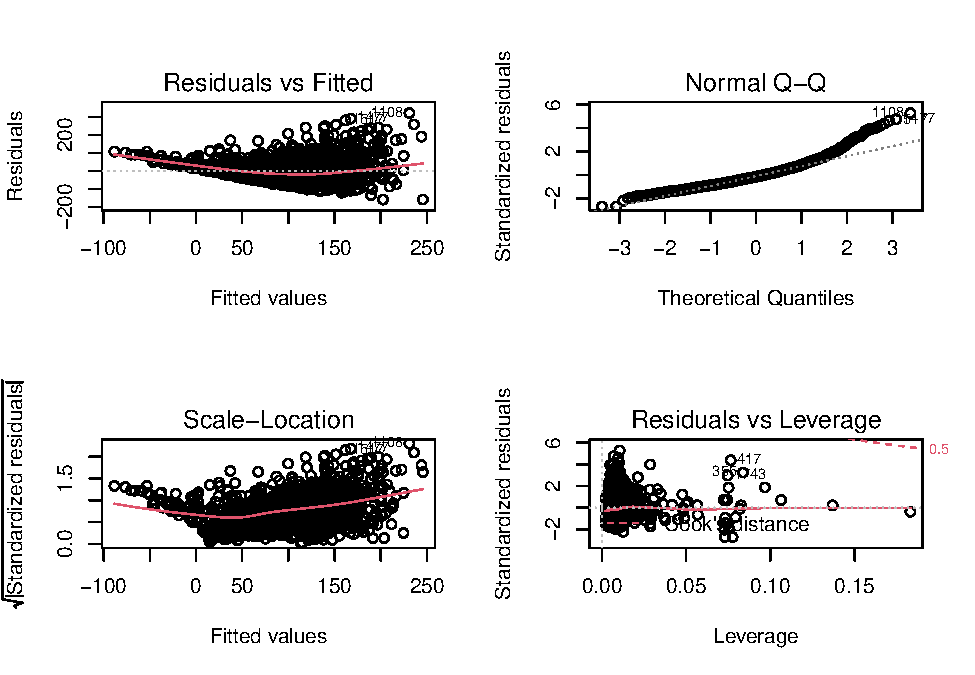
\includegraphics{Final_Project_1_files/figure-latex/unnamed-chunk-9-1.pdf}

\begin{verbatim}
##    X.Homocedasticity. b...0.05 X.Normality. c...0.05 X.Uncorrelated.Errors.
## BP    Homocedasticity    FALSE    Normality    FALSE    Uncorrelated Errors
##    d...0.05
## BP    FALSE
\end{verbatim}

\begin{verbatim}
## [1] b
## <0 行> (或0-长度的row.names)
\end{verbatim}

\begin{verbatim}
##          3          9         35         38         42         43         45 
## 0.18312369 0.01993036 0.02084889 0.02909985 0.02120462 0.02016636 0.01957692 
##         59         60         65         67         73        112        118 
## 0.02778616 0.02873632 0.02280094 0.04509421 0.05684717 0.02384532 0.02513578 
##        119        148        212        250        260        264        297 
## 0.02561832 0.04775556 0.02202594 0.01983728 0.07229409 0.02603939 0.03053323 
##        347        355        364        365        372        375        404 
## 0.02136388 0.08376838 0.02120852 0.04800714 0.03052893 0.02213194 0.02044289 
##        409        417        423        465        470        575        608 
## 0.04888755 0.07645773 0.02899026 0.02330743 0.01974735 0.02305260 0.02132032 
##        618        659        664        702        717        725        734 
## 0.03280053 0.07335589 0.07415222 0.02154804 0.01978184 0.02197048 0.02104081 
##        737        758        760        792        808        894        918 
## 0.08265230 0.07757221 0.02815190 0.04180265 0.02611715 0.02164709 0.02029063 
##        933        934        939        943        944       1017       1018 
## 0.02844410 0.04995945 0.01991536 0.03709670 0.04839376 0.07291344 0.07278236 
##       1019       1039       1040       1044       1064       1065       1077 
## 0.07320367 0.10636050 0.03250507 0.07316761 0.01984485 0.01984594 0.02111622 
##       1079       1098       1099       1119       1125       1128       1129 
## 0.09675365 0.02018495 0.02925196 0.02134172 0.02862577 0.02008693 0.01977021 
##       1130       1175       1183       1292       1362       1370       1375 
## 0.03647560 0.02881126 0.02004238 0.05664320 0.02051762 0.02092169 0.07448111 
##       1428       1429       1434       1449       1454       1457       1463 
## 0.03298086 0.03492779 0.01996232 0.01966219 0.07518163 0.02553009 0.07930188 
##       1485       1499       1500       1555       1592       1654       1677 
## 0.02054096 0.08190632 0.13694349 0.02033825 0.03754080 0.01992540 0.02158615 
##       1703       1727       1743       1772       1792       1797 
## 0.02238124 0.05105359 0.07468200 0.07520319 0.01981613 0.02760467
\end{verbatim}

\begin{verbatim}
##             b d        c
## 417  4.416884 > 4.152357
## 1108 5.333325 > 4.152357
## 1477 4.792634 > 4.152357
## 1517 4.647787 > 4.152357
## 1518 4.233889 > 4.152357
\end{verbatim}

\begin{verbatim}
## Analysis of Variance Table
## 
## Response: Avg_Day_PM2.5
##                Df  Sum Sq Mean Sq  F value    Pr(>F)    
## Date_D          1    1339    1339   0.3577 0.5499001    
## Avg_Day_DEWP    1  188302  188302  50.3013 2.073e-12 ***
## Avg_Day_TEMP    1 2395516 2395516 639.9164 < 2.2e-16 ***
## Avg_Day_PRES    1  244962  244962  65.4370 1.275e-15 ***
## Max_Day_LWS     1  232063  232063  61.9912 6.801e-15 ***
## Max_Day_LS      1   38629   38629  10.3189 0.0013463 ** 
## Max_Day_LR      1  293980  293980  78.5312 < 2.2e-16 ***
## Max_Day_CBWD    3  110235   36745   9.8158 2.076e-06 ***
## Year            1   44499   44499  11.8871 0.0005818 ***
## Month           1   64290   64290  17.1739 3.612e-05 ***
## Day             1   22101   22101   5.9038 0.0152314 *  
## Residuals    1420 5315745    3743                       
## ---
## Signif. codes:  0 '***' 0.001 '**' 0.01 '*' 0.05 '.' 0.1 ' ' 1
\end{verbatim}

\end{document}
